
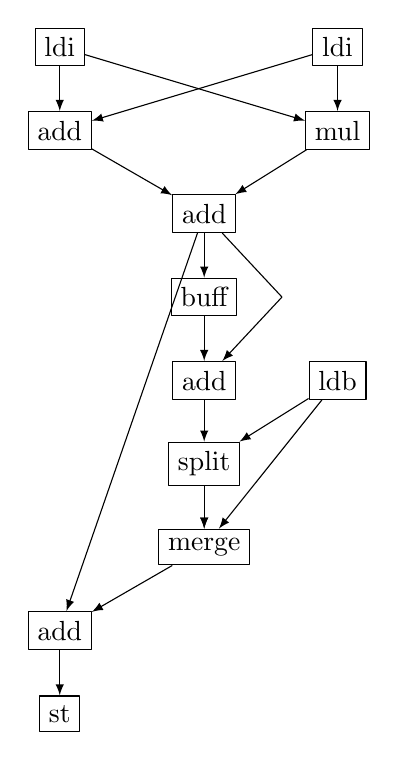
\begin{tikzpicture}[>=latex,line join=bevel,]
%%
\node (ldb) at (200bp,130bp) [draw=black,rectangle] {ldb};
  \node (h_st) at (100bp,10bp) [draw=black,rectangle] {st};
  \node (add4) at (100bp,40bp) [draw=black,rectangle] {add};
  \node (add3) at (152bp,130bp) [draw=black,rectangle] {add};
  \node (add2) at (152bp,190bp) [draw=black,rectangle] {add};
  \node (add1) at (100bp,220bp) [draw=black,rectangle] {add};
  \node (ldi2) at (200bp,250bp) [draw=black,rectangle] {ldi};
  \node (ldi1) at (100bp,250bp) [draw=black,rectangle] {ldi};
  \node (merge) at (152bp,70bp) [draw=black,rectangle] {merge};
  \node (split) at (152bp,100bp) [draw=black,rectangle] {split};
  \coordinate (aux) at (180bp,160bp);
  \node (mul1) at (200bp,220bp) [draw=black,rectangle] {mul};
  \node (buff) at (152bp,160bp) [draw=black,rectangle] {buff};
  \draw [->,solid] (ldi2) -- (add1);
  \draw [->,solid] (add4) -- (h_st);
  \draw [->,solid] (add2) -- (buff);
  \draw [->,solid] (aux) -- (add3);
  \draw [->,solid] (ldb) -- (split);
  \draw [->,solid] (buff) -- (add3);
  \draw [->,solid] (ldb) -- (merge);
  \draw [->,solid] (ldi2) -- (mul1);
  \draw [->,solid] (ldi1) -- (mul1);
  \draw [solid] (add2) -- (aux);
  \draw [->,solid] (merge) -- (add4);
  \draw [->,solid] (mul1) -- (add2);
  \draw [->,solid] (add3) -- (split);
  \draw [->,solid] (split) -- (merge);
  \draw [->,solid] (split) -- (merge);
  \draw [->,solid] (ldi1) -- (add1);
  \draw [->,solid] (add1) -- (add2);
  \draw [->,solid] (add2) -- (add4);
%
\end{tikzpicture}

